\par Durant notre stage de fin d’études, nous avons eu la chance de travailler au sein d’une équipe opérationnelle et bien organisée, dont les membres sont dotés de l’esprit d’équipe, d’entre-aide et du sens d’initiative et de créativité.
\par Dans la présente Section, on va découvrir ces équipes là et les projets aux quel j'ai eu la chance de contribuer.

\begingroup
\let\clearpage\relax
\chapter{OST/ITS/INV/MDM}\label{mdm}
\endgroup

\par Comme toutes les grandes multinationales, Amundi AM recense un nombre incalculable de départements, de secteurs ou d'équipes. Dans le chapitre suivant, je vais décrire l’organisation générale des deux équipes où j’ai effectué mon stage, en suivant une approche descendante.
\\~\\

\section{OST: Operations Services \& Technologies}

\par Amundi AM est subdivisée en plusieurs entités principales (nommée Divisions), on retrouve notamment les départements administrant le groupe Amundi AM (par exemple le département DGL, présidé par Mr. Perrier Yves, président et directeur général du groupe Amundi), les départements relatifs au relations clients Amundi AM (par exemple INS: Institutional Clients Division, RET: Retail Clients Division \dots). Ensuite on retrouve les divisions responsables des activités d'Amundi AM, a savoir BSC (Business Support \& Control) et OST (Operations services \& Technologies). 
\par Présidé par Mr. Lesage Guillaume, cette division regroupe les différents départements essentiels a la gestions d'actifs, activité principale d'Amundi AM. On retrouve par exemple le service NEG (Negociation), ASM (Asset Servicing Management), ASV (Amundi Services) et AFN (Amundi Finance). En plus de ces départements, la division contient aussi ITS (Amundi Technology, IT Services), département auquel j'ai été affecté, qui contient à son tour plusieurs services. 
\clearpage
\section{ITS: Amundi Technology, IT Services}

\begin{figure}[ht]
    \centering
    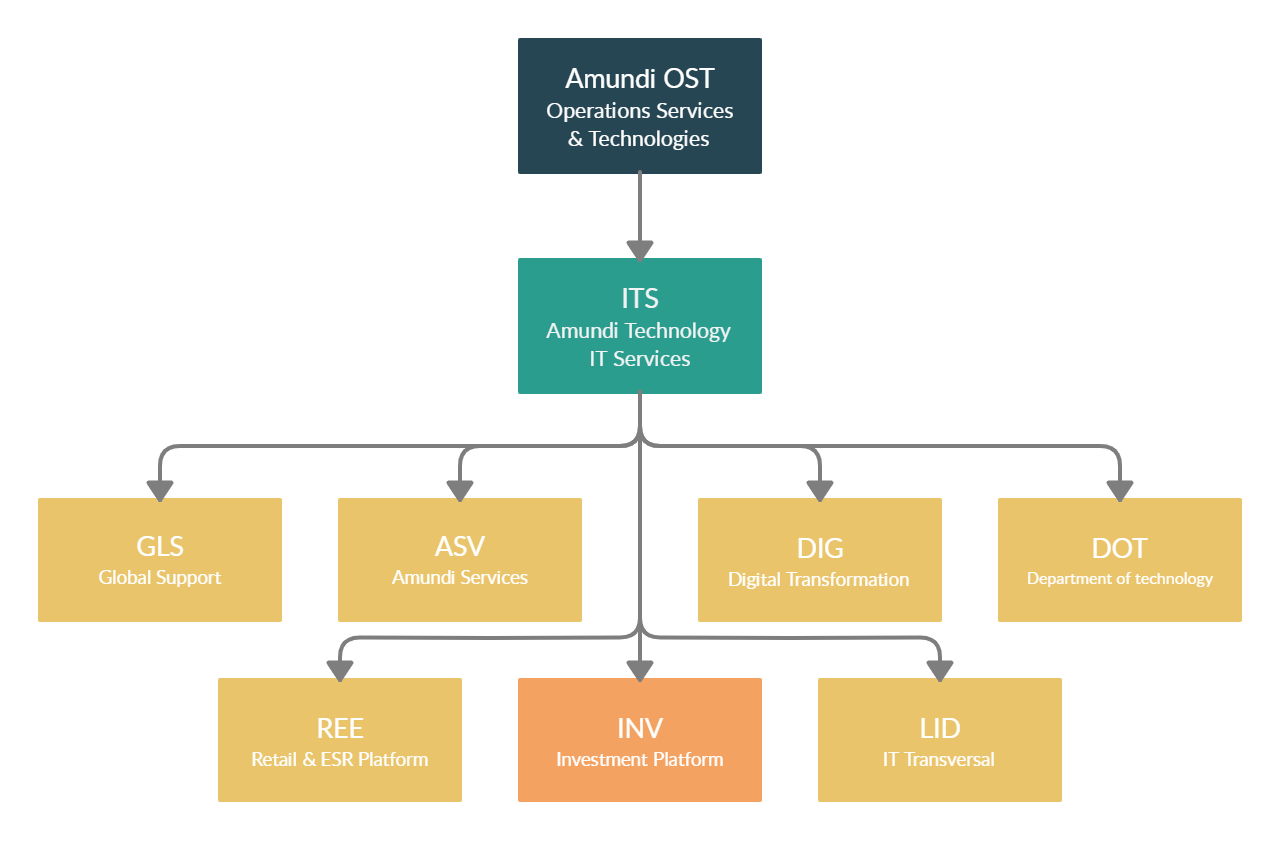
\includegraphics[width=\columnwidth]{img/Org ITS.png}
    \caption{Organisation ITS}
    \label{fig:its}
\end{figure}

\par Le département ITS, comme le nom l'indique, est le département responsable de tout ce qui est service IT. Il est composé de sept services comme le montre la figure \ref{fig:its} ci-dessus: 
\begin{itemize}
    \item GLS (Global Support): la branche d'Amundi ITS basé à Dublin (Irlande) subdivisée en deux services, DHB (Dublin Hub and Intl. Development)\& DOT (Department of technology: Dublin Hub and infrastructure)
    \item ASV (Amundi Services): Amundi services (cf. Part I. Chapitre II.)
    \item DIG (Digital Transformation): Service mutualisé avec le département BSC (Business support and control) chargé de la transformation et communication digitale.
    \item DOT (Department of technology): regroupe les équipes qui travaillent sur le côté hardware (architecture, infrastructure et réseaux), Frameworks internes (dont un que j'ai eu la chance d'utiliser dans un projet) et gestion de base de données. 
    \item REE (Retail \& ESR Platform): Service gérant deux applications Amundi AM majeurs, Alto Retail et ESR. 
    \item LID (IT Transversal): Leading IT Department
    \item INV (Investment Management Platform): Service qui est subdivisé en plusieurs équipes, responsables de plusieurs applications client et interne Amundi AM. Service auquel j'ai été affecté et qu'on va détailler dans la prochaine section
\end{itemize}

\section{INV: Investment Management Platform}
\par Comme c'est déjà mentionné dans la précédente section, le service INV est subdivisé en plusieurs équipes (comme le montre la figure \ref{fig:inv} ci-dessous).\\
\begin{itemize}
    \item EAX: Entreprise Architecture \& UX Design, Équipe qui ce charge de tout ce qui design et maquettes d'applications (User Interface, User Experience) (Notamment utilisé dans le projet Alto Investment Research cf. Partie II. Chapitre II. Section 2) 
    \item FOA: Front Office \& Analysis, Équipe qui se charge des projets Front office (cf. Partie I. Chapitre II. Section I. Sous-Section "Organisation d'un Asset Manager")
    \item RIS: Risk Development
    \item DHB: Dublin Hub Development, précédemment cité dans la Section 2 du Chapitre I. de la partie II. est l'équipe INV basée a Dublin (Irlande). Elle se compose principalement du projet PKC (Position Keeping \& Control) 
    \item INS: Institutional 
    \item TTP: Trading \& MO Trade Processing 
    \item MDM: Master Data Management, Équipe a laquelle je suis affecté, la prochaine section de ce chapitre essayera de détailler ses missions, applications gérés, et périmètre de fonctions.
\end{itemize}
\par Chaque équipe gère des applications essentiels au activités d'Amundi AM.
\begin{figure}[ht]
    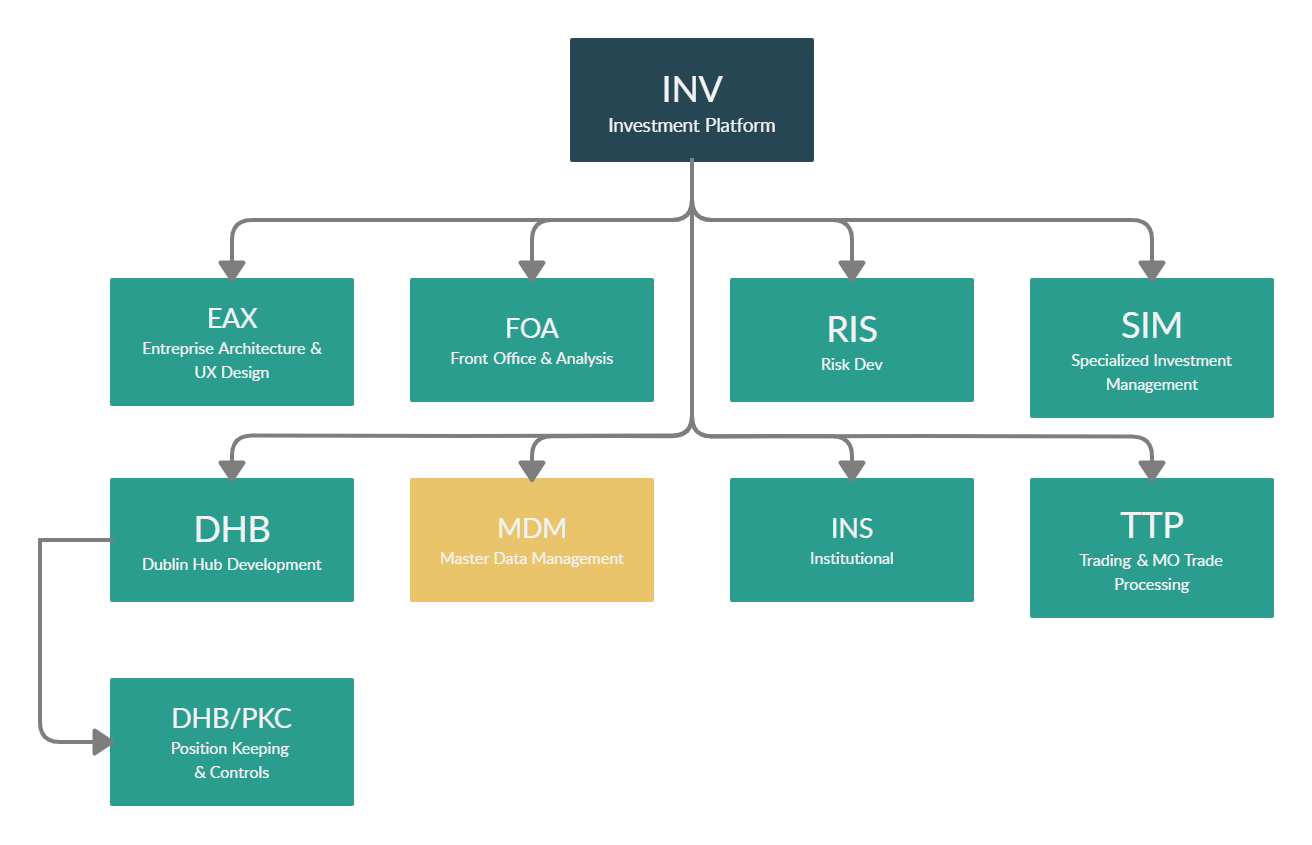
\includegraphics[width=\columnwidth]{img/Org INV.png}
    \caption{Organisation INV}
    \label{fig:inv}
\end{figure}

\section{MDM: Master Data management}
\par MDM, ou Master Data Management, est le département responsable de toutes les application gérant les données utilisé par le métier Amundi (Exemple: portefeuilles, positions, données marchés\dots)(communément appelé Master Data). L'équipe est managé par Mr. Lionel Fournier et regroupe plus de trente-cinq ingénieurs dont plusieurs MOE.
\par On dénombre pour le moment sept projets majeurs:
\begin{itemize}
    \item Life : C'est le projet d'implémentation de DataHub, au sein d'Amundi, en vue d'une gestion des référentiels tiers en valeurs et indices. Ce projet a aussi pour but de traiter l’obsolescence ainsi que l'optimisation d’une partie du SI Référentiels.
    \item Medco: ou MediaPlus-core est l'un des projets les plus importants de MDM. C'est le serveur de diffusion, en date du jour, de données principale, notamment pour les portefeuilles et instruments (et tout donnée relatifs). Le but étant de Sérialiser et cacher (transformer en Caches) des objets qui sont des mappings JAVA d'une ou plusieurs tables de base de données. Ceci permet d'avoir un accès direct a ces donnes via l'API MediaPlus-core pour tout client du serveur.
    \item Refgt: ou Referential Gate est un autre serveur de diffusion, mais pour le coup, en date passée. Le serveur récupère ses données depuis plusieurs sources notamment Medco ainsi que des différentes tables de bases de données, pour les historiser. Le serveur permet aussi d'écrire certain types de data dans les différentes tables de bases de données. 
    \item Hubref: ou Refrential Hub, est un serveur de routage, il permet selon le besoin de récupérer la data depuis RefGate ou Medco et de la diffuser a son tour. Ce serveur est notamment utilisé par plusieurs applications front comme Alto Investment Research.
    \item Atlas: Cet application Master Data Management se charge de collecter, intégrer, administrer et diffuser la data qui provient des partenaires d'Amundi AM.
    \item Indice: est une application/serveur qui gère tout autour de deux types d'instruments financier, les indices et benchmarks. 
    \item Alto Investment Research - Refrential Widgets : Alto (Amundi Leading Technologies and Operations) Investment Research est une application subdivisée entre 3 équipes, une partie pour l'équipe appartenant à ITS/DOT/COR (équipe qui se charge du développement du Framework Maestro, Framework sur lequel est basé l'application), une partie pour l'équipe appartenant à ITS/INV/FOA (équipe en charge de différents types de Data) et la partie assignée à l'équipe ITS/INV/MDM, la partie sur la quelle on gère la data reçu par Hubref.
\end{itemize}

\par En plus de ces sept projets on dénombre plusieurs plus petit projets, ou des projets dont le périmètre de fonctions est plutôt éloigné du contexte de mon stage de fin d'études, on peut notamment citer : MDBM, MDQC, FundLife, DQC, Libra \dots   
\par De mon coté, j'ai été assigné au projet MediaPlus-Core puis au projet Alto Investment Research sur la partie Referential Widgets.
\par Le chapitre suivant apportera plus d'informations sur les deux projets, ainsi que des schémas expliquant le fonctionnement et l'environnement technique de chaque projet.


\chapter{Projets}
\par Durant le présent chapitre, on essayera de projeter plus d'informations sur les deux projets auquel j'ai eu la chance d'être affecté, à savoir MediaPlus-core et Alto Investment Research. On présentera chaque projet, son utilité, ses fonctions, son architecture ainsi que son environnement technique.
\section{MediaPlus-Core}
\par Comme c'est mentionné dans la Partie II. Chapitre I. Section 4, "MediaPlus-core est l'un des projets les plus importants de MDM. C'est le serveur de diffusion, en date du jour, de données principale, notamment pour les portefeuilles et instruments (et tout donnée relatifs). Le but étant de Sérialiser et cacher (transformer en Caches) des objets qui sont des mappings JAVA d'une ou plusieurs tables de base de données. Ceci permet d'avoir un accès direct a ces donnes via l'API MediaPlus-core pour tout client du serveur." 
\par MediaPlus-Core, est un serveur de cache. On récupère de la data de la base de donnée DECALOG (Un système de gestion de base de données basé sur des serveurs Sybase ASE Adaptive Server Enterprise), on les transforme en cache pour on les exposer soit par EJB (Jakarta Enterprise Beans, anciennement Enterprise JavaBeans), soit par webservice REST.
\clearpage
\subsection{Architecture applicative}
\begin{figure}[ht]
    \centering
    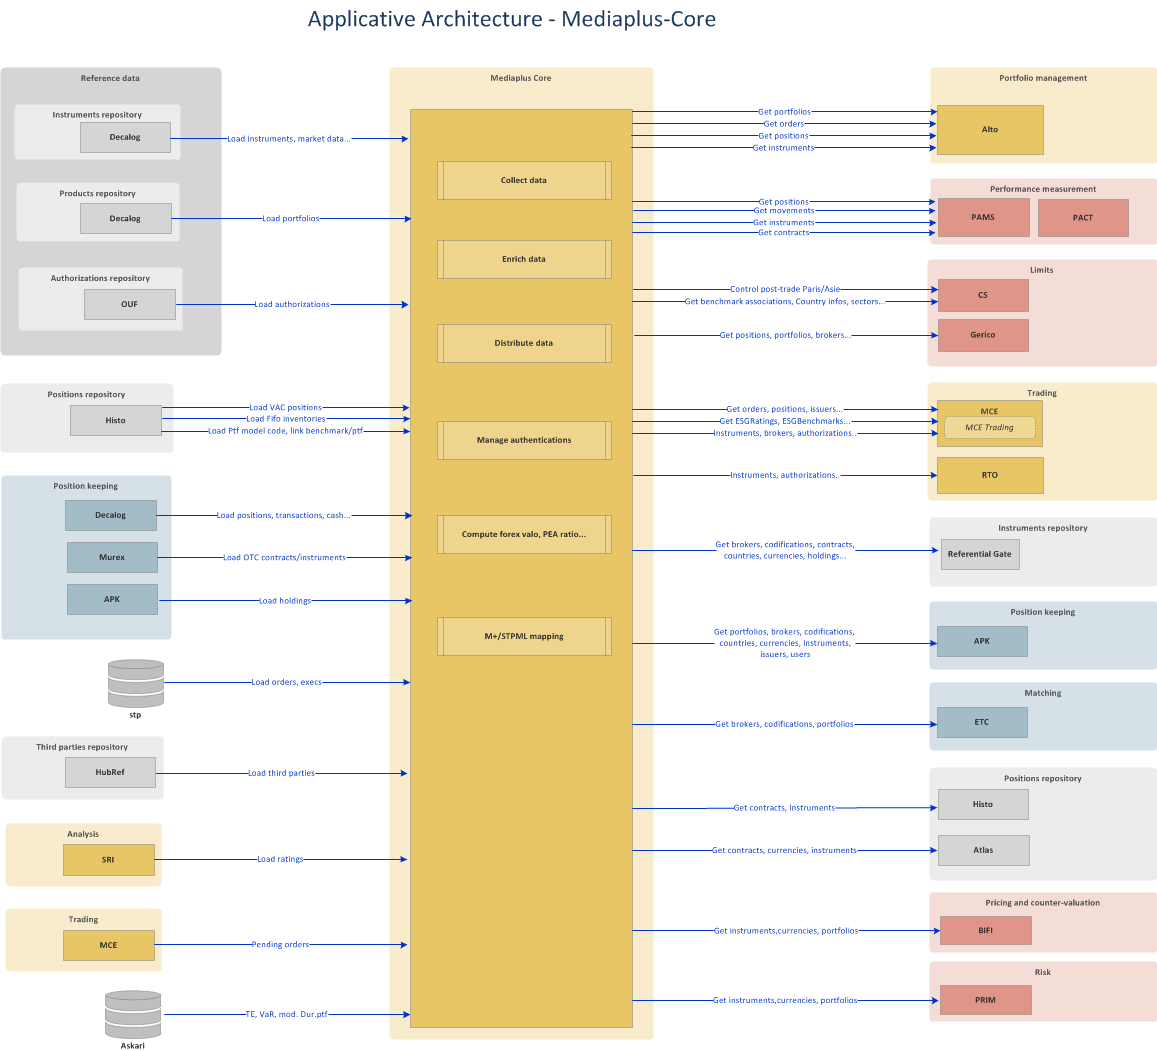
\includegraphics[width=\columnwidth]{img/Architecture Medco.png}
    \caption{Architecture applicative Medco}
    \label{fig:medcoArch}
\end{figure}
\par Sur la figure \ref{fig:medcoArch}, on retrouve a gauche les sources de données subdivisés en segments relatifs au type de donnée. Par exemple on retrouve les données référentiels extraite depuis DECALOG (pour les données instruments et produits), les données de position récupéré depuis DECALOG, une Base de donnée HISTO (Un autre type de base de données), ou l'application APK (Amundi Position Keeping) etc\dots
\par Au milieu on retrouve les principales fonctions de Medco à savoir le traitement de données (Collecte, Transformation et Distribution), la gestion d'authentification et finalement la réalisation de mapping MediaPlusObject, OpenAML et STPML (Plus de détails et d'explications dans la partie III.).
\clearpage
\par Sur la droite on retrouve les sorties, ou les services dont le fonctionnement repose sur Medco. On retrouve par exemple l'ensemble des applications Alto où Medco fournit l'ensemble des informations relatifs au positions, instruments, ordres et portefeuilles; Refgate où Medco fournit un très grand nombre de données primordiales à l'historisation de donnée qu'effectue Refgt; Ainsi que plusieurs autres serveurs/Application tel Hubref, Atlas, APK\dots
\par Comme le montre la figure \ref{fig:medcoArch}, Medco fait partie des plus importants serveurs centraux Amundi vu le nombre d'entrées et sorties mais aussi de la criticité de diffusion de ces données. En effet hormis le fait que les informations soient critiques et sensibles, chaque retard de diffusion d'information peut rendre cette dernière inutilisable, obsolète.  
\par La criticité viens aussi du fait que Medco diffuse la donnée pour des serveur/applications qui à leur tour se charge de la diffuser pour d'autres applications (Ex: RefGate) ou qui se charge du routage de donnée (Ex: Hubref) donc si le serveur Medco ne réussi pas à diffuser l'information, plusieurs services et applications au sein d'Amundi ITS seront inutilisable.

\subsection{Architecture Technique}
\hfill \break
\begin{figure}[ht]
    \centering
    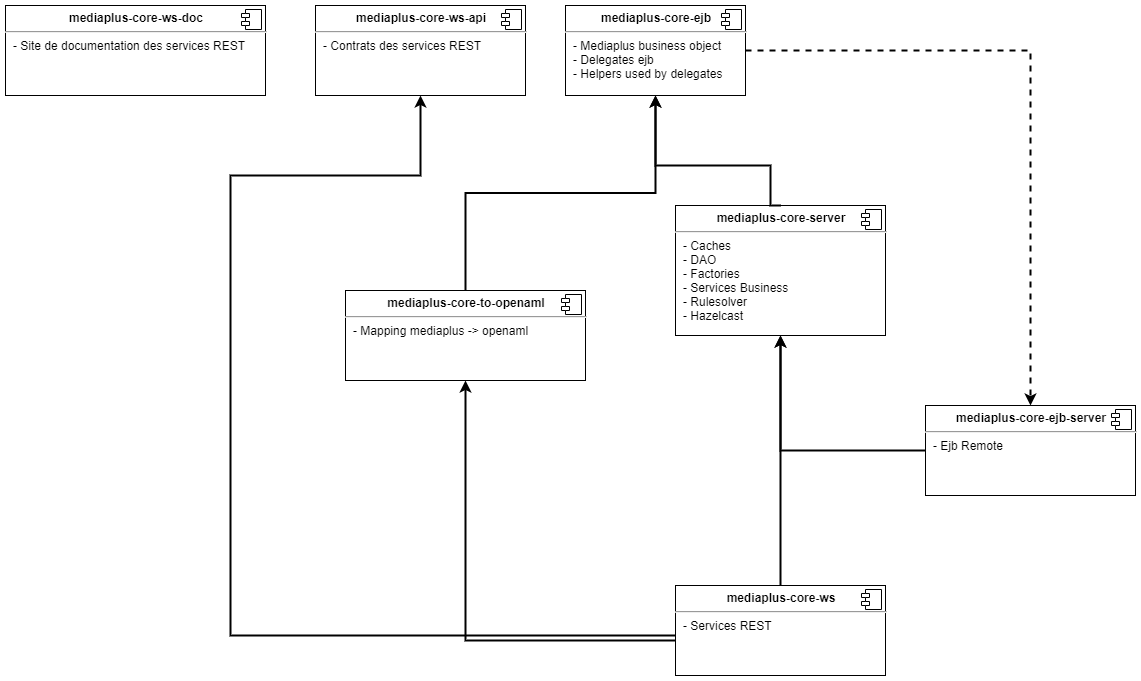
\includegraphics[width=\columnwidth]{img/medco-arch.png}
    \caption{Architecture Technique Medco}
    \label{fig:medcoArchTech}
\end{figure}
\pagebreak
\par Comme le montre la figure \ref{fig:medcoArchTech}, MediaPlus-Core se subdivise en sept sous projets:
\begin{itemize}
    \item Mediaplus-core-server: Représente le cœur du projet MediaPlusCore, il contient les objets et méthodes relatif au cache Medco, la partie DAO  et accès au bases de données, les factories pour créations d'objets, Hazelcast (utilisé pour la mise en cache), Rulesolver pour MediaPlus(à voir dans la partie III.), etc\dots
    \item Mediaplus-core-ejb: Comme le montre le nom, cette partie est responsable de tout ce qui est EJB sur Medco. Elle contient les MediaPlusObject ou les Objets Métiers MediaPlus.
    \item Mediaplus-core-ejb-server: Est responsable de la diffusion de la partie Mediaplus-core-ejb précédemment cité. Elle contient entre autres les remote Ejb.
    \item Mediaplus-core-to-OpenAML: Cette partie est responsable de la conversion d'objets MediaPlus en mappings OpenAML (à voir dans la partie III.)
    \item Mediaplus-core-ws: SousProjet qui contient toute la partie responsable des services REST du projet MediaPlus-core.
    \item Mediaplus-core-ws-api: Partie responsable des endpoints de l'API programmée et créé par la partie Mediaplus-core-ws. Elle est responsable de la diffusion de donnée sous deux formats : OpenAML et STPML (obsolète)
    \item Mediaplus-core-ws-doc: Destiné aux autres équipes IT et Métiers, contient la documentation complete de tout les webservice REST qu'offre MediaPlusCore
\end{itemize}

\par Tout les projets et sous projets sont développé par du JAVA 7. Depuis quelques mois, l'équipe est en phase de transition des projets vers du JAVA 8.
\par Plus de détails concernant d'autres technologies utilisé, ainsi qu'une architecture plus détaillée, seront apporté dans la partie III. de ce présent rapport.
\par On passe à présent à la deuxième partie de ce chapitre, partie qui traite le projet Alto Investment Research.
\pagebreak
\section{Alto: Amundi Leading Technologies \& Operations}
\begin{figure}[ht]
    \centering
    
\includegraphics[width=\columnwidth]{img/Alto.png}
    \caption{Logo Alto}
    \label{fig:altoLogo}
\end{figure}
\par Alto, l'abréviation d'Amundi Leading Technologies \& Operations, est l'un des plus grands projets d'Amundi AM, utilisé par une très grade partie des ingénieurs métier Amundi AM. L'une des plusieurs applications Front Office, elle reste la seule attribuée à l'équipe ITS/INV/MDM.
\par Le projet est subdivisé en plusieurs parties. Pour des raisons de confidentialité, on traitera uniquement le projet Alto Investment Research.
\subsection{Alto Investment Research}
\par Alto Investment Research, anciennement Alto Master Data, est la partie du projet Alto chargé de traiter la data diffusé par le département MDM, la master data comme définie dans la Partie II. Chapitre I. Section 4.
\par Le projet est sous forme d'une application Front Office, ou l'utilisateur, en fonction de trois types d'entités financière (Assets, Issuers et Portfolios), peut visualiser plusieurs paramètres financiers, des graphes et tableaux contenant les données diffusé par les différents serveurs/applications. Cette application est notamment utilisé par les ingénieurs métiers Amundi AM (Ex: Traders).
\par L'application contient plusieurs widgets (cf. figure XXXX). La création, maintenance et gestion de ces widgets est subdivisée en deux partie: Master Data SRI (géré par l'équipe GES/RIV (pour Responsible Investments) et l'équipe ITS/INV/FOA), et Referential Widgets (géré par l'équipe ITS/INV/MDM), partie sur laquelle je travaillait.

\subsection{Masterdata SRI ESG}
\par MasterData SRI ESG, abréviation pour Master Data for Socially Responsible Investing \& Environmental, social and corporate governance, est la partie du projet Alto Investment Research contenant les widgets exposant de la data relative aux investissement socialement responsable et critères environnementaux et sociaux de gouvernance d'entreprises.
\par Par exemple on retrouve des widgets exposant les émissions Carbonne des entreprises (SRI) (cf. figure \ref{fig:sri}) 
\par Sur la figure \ref{fig:esg}, on retrouve un widget de type ESG montrant un classement et donnant une note à une entreprise selon son respect des critères environnementaux et sociaux de gouvernance d'entreprises.
\par Le développement, maintenance, gestion et administration de ces widgets sont délégué à une autre équipe ITS, une équipe chargée de gérer plusieurs applications front office et de réaliser des analyses sur la data, l'équipe ITS/INV/FOA, FOA pour Front Office \& Analysis.
\begin{figure}[ht]
    \centering
    \subfloat[\centering Widget SRI]{{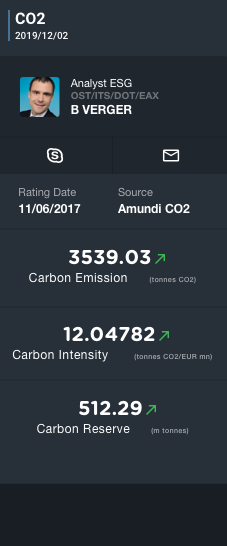
\includegraphics[width=5cm]{img/SRI.png} \label{fig:sri}}}%
    \qquad \qquad \qquad \qquad
    \subfloat[\centering Widget ESG]{{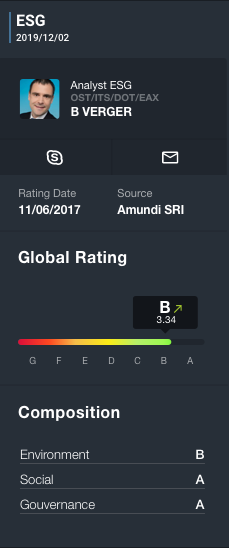
\includegraphics[width=5cm]{img/ESG.png} \label{fig:esg} }}%
    \caption{Exemples de Widgets Masterdata SRI ESG}
\end{figure}
\clearpage
\subsection{Referential Widgets}
\par Referential Widgets est la section du projet Alto Investment Research contenant les widgets exposant la master data ne figurant pas dans les widgets ESR et SRI. Communément appelé Referential Data, ces données sont indispensables au métier Amundi AM.
\par Les entités représenté sur ces widgets sont subdivisée en trois types d'entités: des Issuers, des Assets et finalement des Portfolios. Chaque types d'entité à une interface ou écrans diffèrent des autres types (Exemple figure \ref{fig:AssetInvision} pour un Asset figure \ref{fig:IssuerMaestro} pour un Issuer).
\par Chaque type d'entité est a son tour potentiellement contenant plusieurs classes (par exemple pour des Assets on peut retrouver des Equity, des Bonds, Derivatives, Index, Fixed Income\dots), sauf qu'ils auront globalement la même interface avec des changements mineurs (exemple: on supprime des champs car leur présence est illogique par rapport à la classe représenté). \\
\begin{figure}[ht]
    \centering
    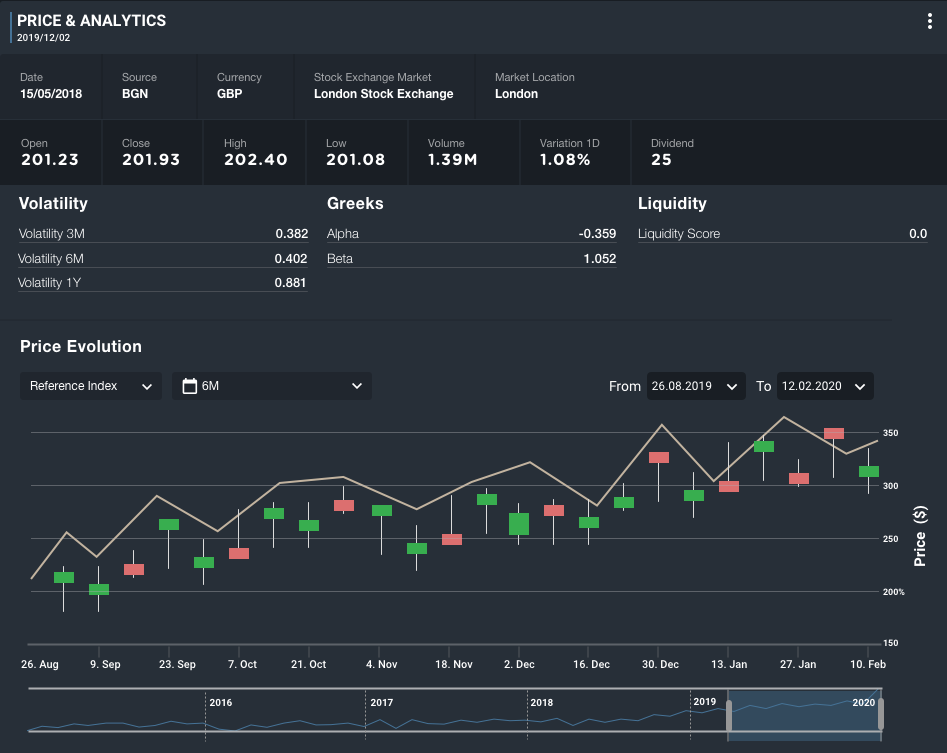
\includegraphics[width=\columnwidth]{img/AssetInvision.png}
    \caption{Exemple de widget Referential - Asset (Equity)}
    \label{fig:AssetInvision}
\end{figure}
\clearpage
\begin{figure}[ht]
    \centering
    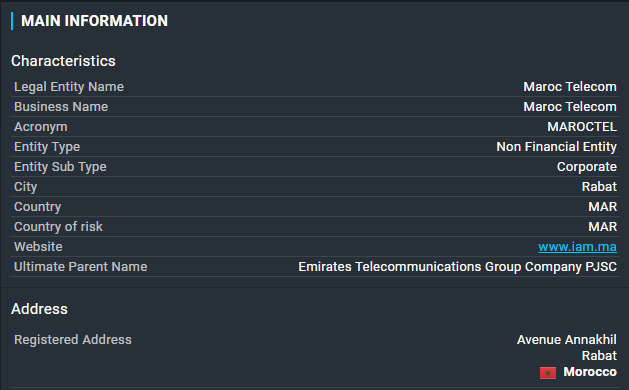
\includegraphics[width=\columnwidth]{img/IssuerWidgetIAM.png}
    \caption{Exemple de widget Referential - Issuer}
    \label{fig:IssuerMaestro}
\end{figure}
\par Sur près de 50 widgets contenu dans l'application Alto Investment Research, les widgets Referentials représentent plus de 85\% des widgets présents, le reste étant constitué de widgets MasterData SRI \& ESG.
\\~\\
\begin{figure}[ht]
    \centering
    
\includegraphics[width=4cm]{img/MAES.png}
    \caption{Logo Maestro}
    \label{fig:maes}
\end{figure}
\par L'application Alto Investment Research, ainsi que les différents widgets Master Data SRI \& ESG et Referential Widgets ont été développé en utilisant la version 5.2.0 puis 5.3.2 du Framework Maestro, un Framework interne d'Amundi-ITS, développé par l'équipe "ITS/DOT/COR Entreprise Framework".
\clearpage
\par Il est basé sur la version 8.2 du Framework Angular, développé par Google LLC, et inclus plusieurs surcouches unifiant toutes les applications front Amundi AM, pouvant parfois faciliter des blocs de code.\\
\begin{figure}[ht]
    \centering
    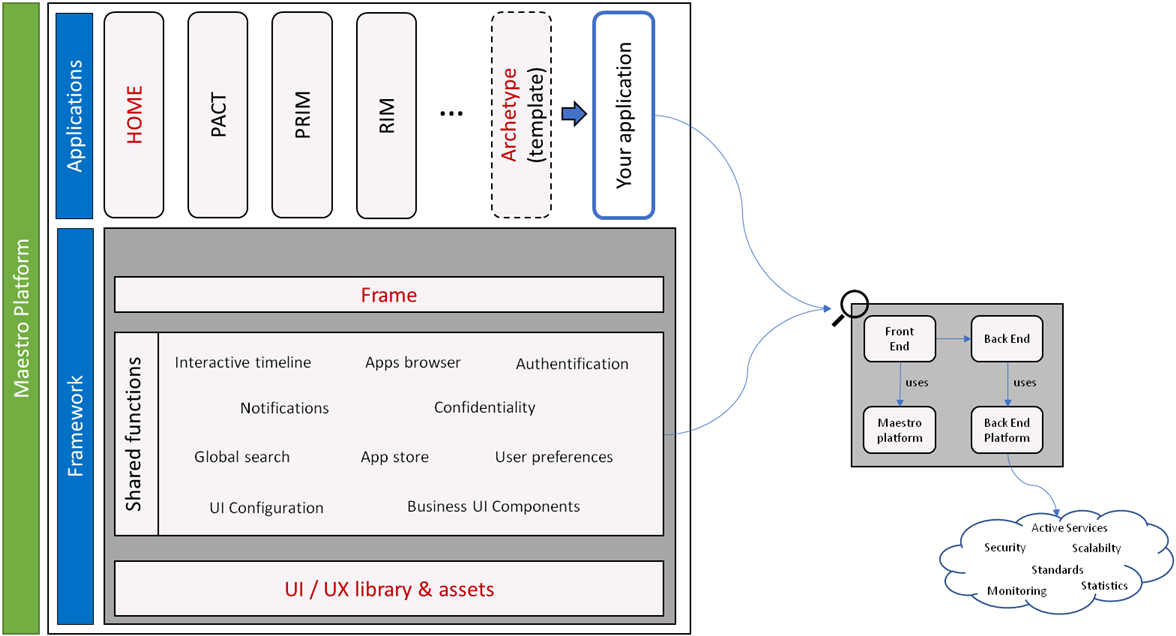
\includegraphics[width=\columnwidth]{img/Maestro.png}
    \caption{Architecture Maestro}
    \label{fig:archMaestro}
\end{figure}

\par L'architecture de Maestro est disponible sur la figure \ref{fig:archMaestro}. Une documentation interne est disponible en interne. Des formations Maestro sont régulièrement organisé par l'équipe "ITS/DOT/COR Entreprise Framework".
\par Sur le projet Alto Investment Research - Referential Widgets, l'équipe était formé de trois ingénieurs : Imad Saine, Dorian Antoine (Tout deux aussi membre de l'équipe MediaplusCore) et moi même. Des réunions sont organisé régulièrement avec Hilmi Sara, MOA Front Office, de l'équipe GES/COO/GIS/MFO, qui se chargeait d'étudier le besoin avec les ingénieurs métiers Amundi AM, l'analyser et par la suite nous proposer une formulation du problème à traiter ou des directives à suivre côté IT MDM.